%%%%%%%%%%%%%%%%%%%%%%%%%%%%%%%%%%%%%%%%%%%%%%%%%%%%%%%%%%%%%%%%%%%%%
% cover.tex - Book Cover for Causal Inference in Marketing
%
% Compile with: pdflatex cover.tex
%%%%%%%%%%%%%%%%%%%%%%%%%%%%%%%%%%%%%%%%%%%%%%%%%%%%%%%%%%%%%%%%%%%%%

\documentclass[a4paper]{article}
\usepackage[margin=0pt, paperwidth=210mm, paperheight=297mm]{geometry}
\usepackage{tikz}
\usetikzlibrary{calc, positioning, shapes.geometric, arrows.meta}
\usepackage{xcolor}
\usepackage[T1]{fontenc}
\usepackage{lmodern}

% Define colors
\definecolor{darkblue}{RGB}{15, 32, 65}
\definecolor{accentblue}{RGB}{65, 105, 225}
\definecolor{lightaccent}{RGB}{100, 149, 237}
\definecolor{goldaccent}{RGB}{218, 165, 32}

\pagestyle{empty}

\begin{document}
\noindent
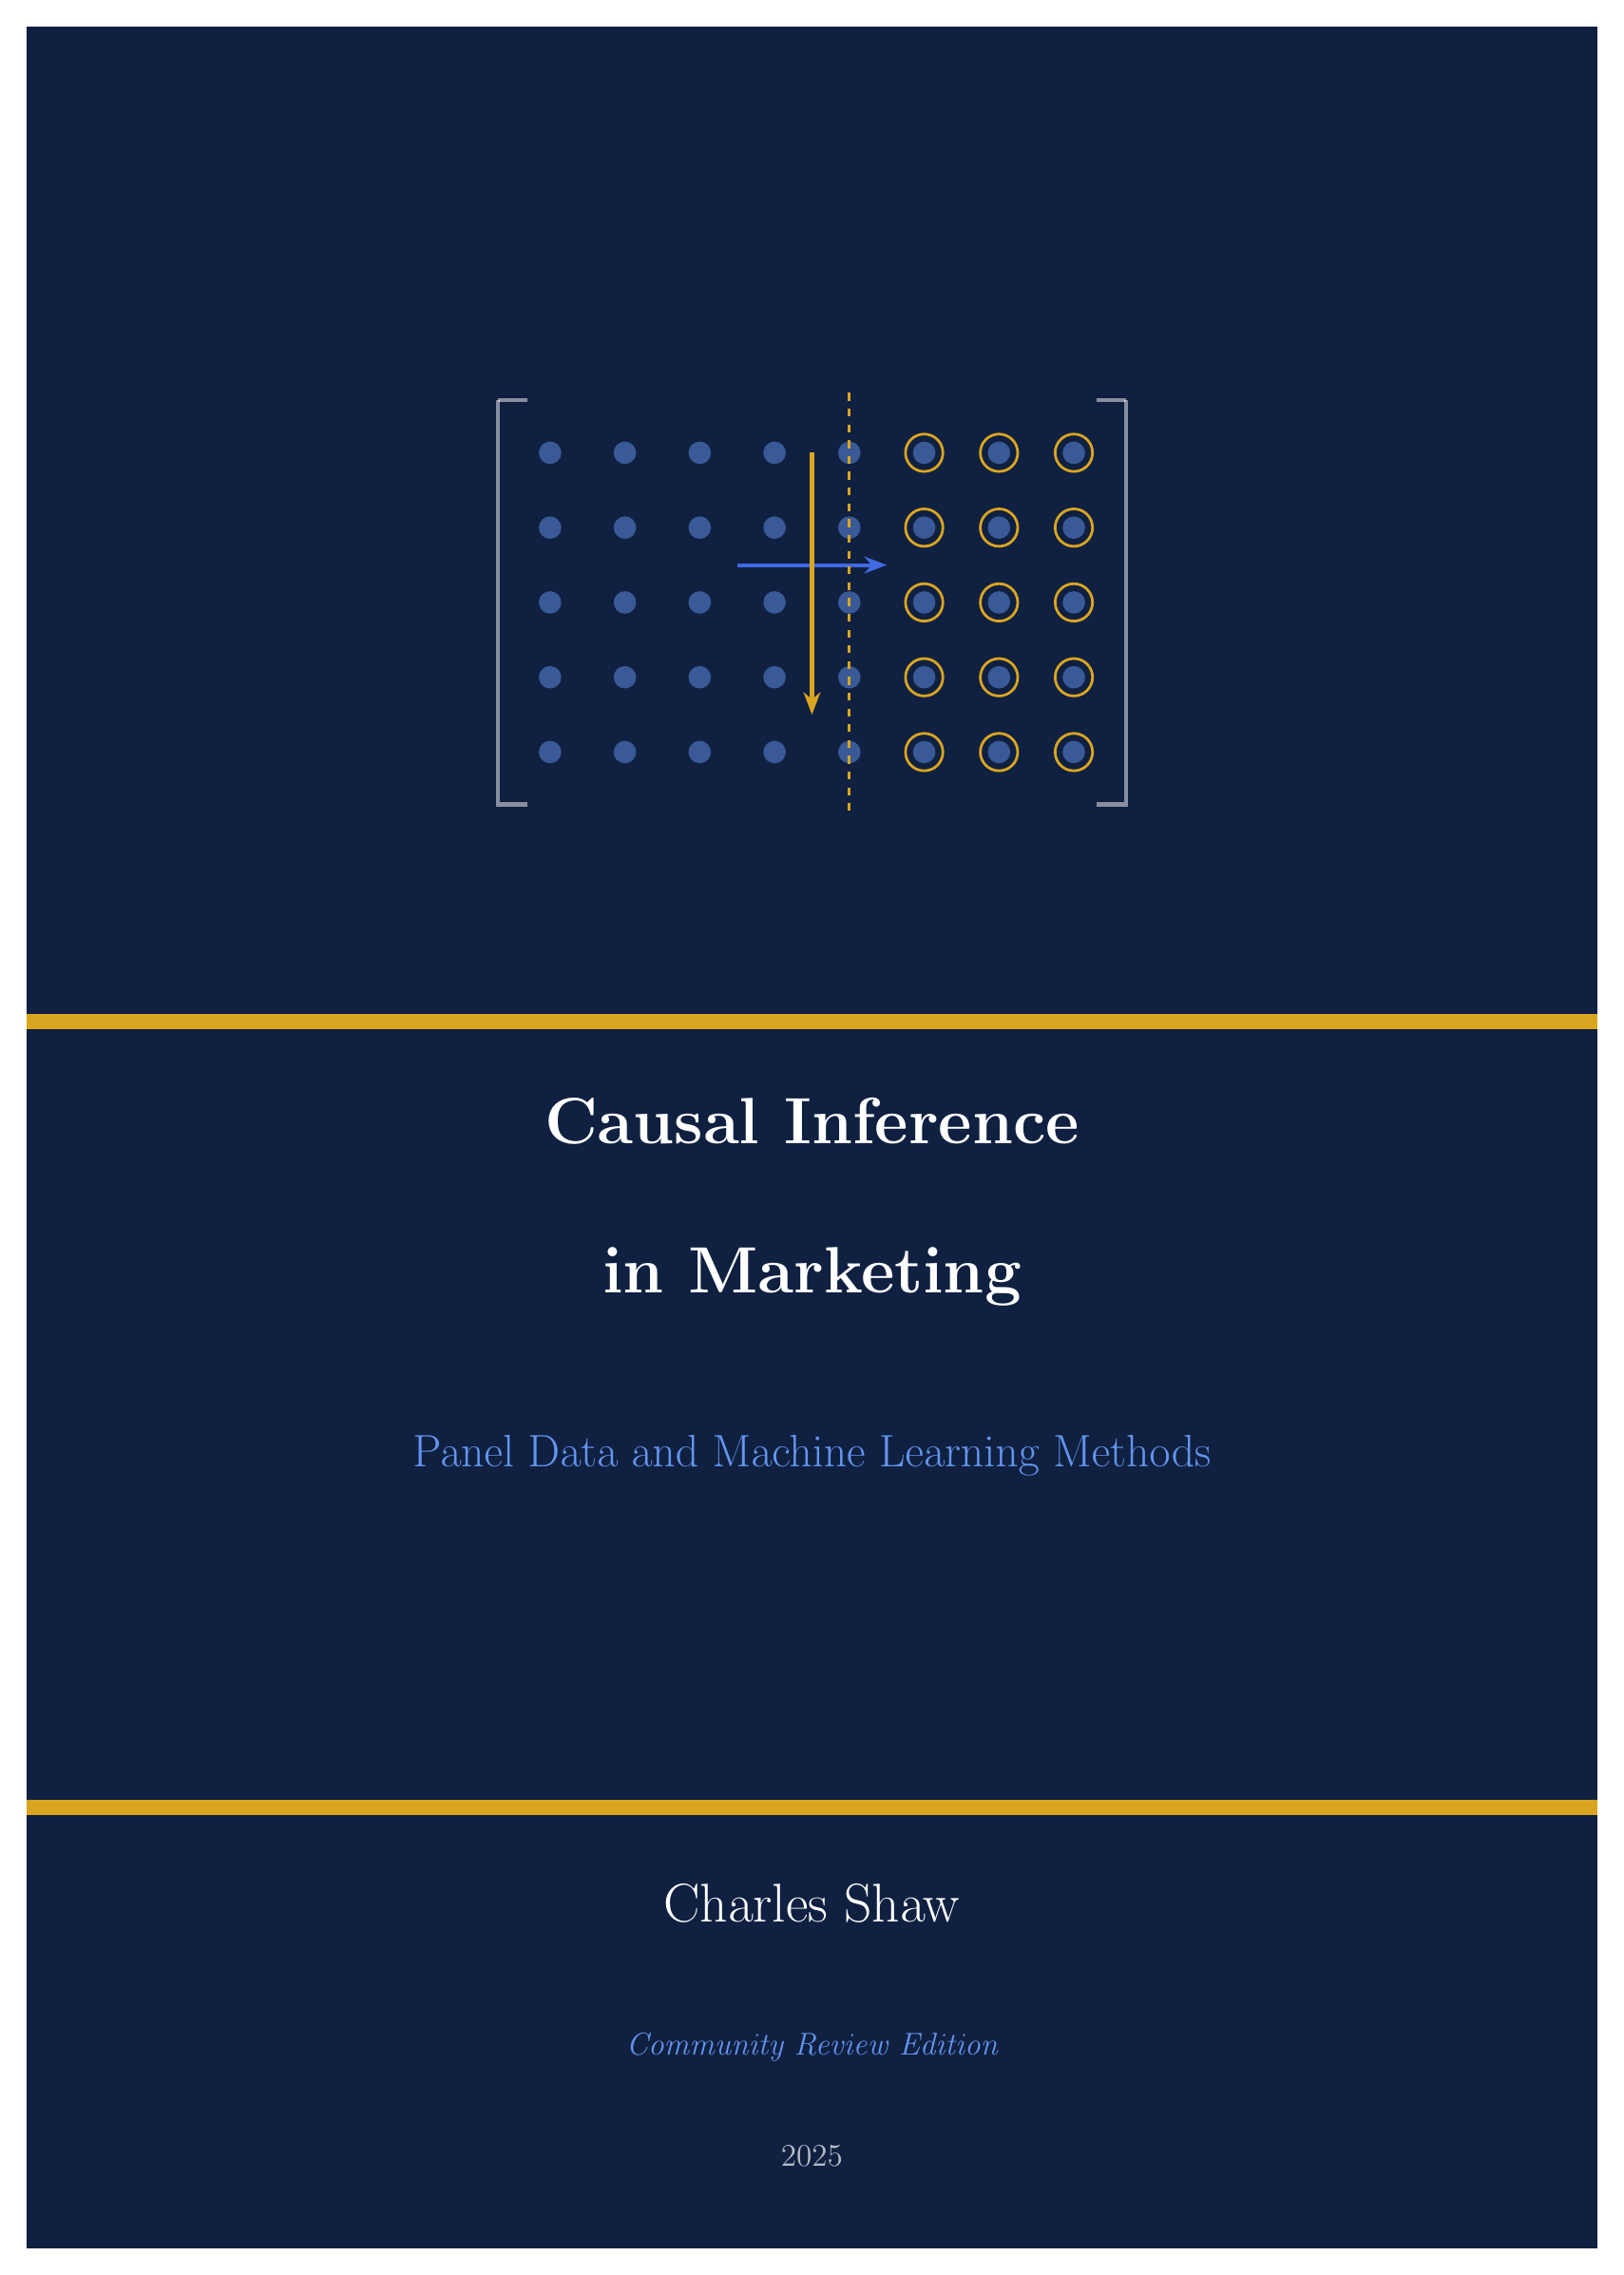
\begin{tikzpicture}[x=1mm, y=1mm]
    % Background - A4 size: 210mm x 297mm
    \fill[darkblue] (0,0) rectangle (210, 297);
    
    % Abstract geometric pattern - representing panel data matrix
    \begin{scope}[shift={(105, 220)}]
        % Grid of nodes representing panel data (units x time)
        \foreach \i in {0,1,2,3,4,5,6,7} {
            \foreach \j in {0,1,2,3,4} {
                \fill[lightaccent, opacity=0.5] 
                    (-35 + \i*10, 20 - \j*10) circle (1.5);
            }
        }
        
        % Causal arrows (treatment effects)
        \draw[-{Stealth[length=3mm]}, accentblue, line width=1.5pt] 
            (-10, 5) -- (10, 5);
        \draw[-{Stealth[length=3mm]}, goldaccent, line width=1.5pt] 
            (0, 20) -- (0, -15);
            
        % Highlight treated units (post-treatment)
        \foreach \j in {0,1,2,3,4} {
            \draw[goldaccent, line width=1pt] 
                (15, 20 - \j*10) circle (2.5);
            \draw[goldaccent, line width=1pt] 
                (25, 20 - \j*10) circle (2.5);
            \draw[goldaccent, line width=1pt] 
                (35, 20 - \j*10) circle (2.5);
        }
        
        % Vertical treatment line
        \draw[goldaccent, dashed, line width=1pt]
            (5, 28) -- (5, -28);
        
        % Matrix brackets
        \draw[white, opacity=0.5, line width=1.5pt] 
            (-42, 27) -- (-42, -27) -- (-38, -27);
        \draw[white, opacity=0.5, line width=1.5pt] 
            (42, 27) -- (42, -27) -- (38, -27);
        \draw[white, opacity=0.5, line width=1.5pt] 
            (-42, 27) -- (-38, 27);
        \draw[white, opacity=0.5, line width=1.5pt] 
            (42, 27) -- (38, 27);
    \end{scope}
    
    % Top decorative line
    \fill[goldaccent] (0, 165) rectangle (210, 163);
    
    % Title
    \node[anchor=north, text=white, font=\fontsize{42}{50}\selectfont\bfseries] 
        at (105, 155) {Causal Inference};
    \node[anchor=north, text=white, font=\fontsize{42}{50}\selectfont\bfseries] 
        at (105, 135) {in Marketing};
    
    % Subtitle
    \node[anchor=north, text=lightaccent, font=\fontsize{18}{22}\selectfont] 
        at (105, 110) {Panel Data and Machine Learning Methods};
    
    % Bottom decorative line
    \fill[goldaccent] (0, 60) rectangle (210, 58);
    
    % Author
    \node[anchor=north, text=white, font=\fontsize{20}{24}\selectfont] 
        at (105, 50) {Charles Shaw};
    
    % Edition note
    \node[anchor=north, text=lightaccent, font=\fontsize{12}{16}\selectfont\itshape] 
        at (105, 30) {Community Review Edition};
    
    % Year
    \node[anchor=north, text=white, font=\fontsize{12}{16}\selectfont, opacity=0.7] 
        at (105, 15) {2025};

\end{tikzpicture}

\end{document}
